\documentclass[9pt,a4paper,oneside]{scrartcl}
\usepackage[latin1]{inputenc}
\usepackage{amsmath}
\usepackage{amsfonts}
\usepackage{amssymb}
\usepackage{makeidx}
\usepackage{graphicx}
\usepackage{booktabs}
\usepackage[
	   style=ieee
	   ]
	   {biblatex}
\usepackage[a4paper,width=170mm,top=18mm,bottom=22mm,includeheadfoot]{geometry}
\usepackage{mathtools}
\usepackage{concmath}
\usepackage[T1]{fontenc}
\usepackage{pgf}
\usepackage{tikz}
\usetikzlibrary{shapes}
\author{}
\title{Ethereum Block}
\date{}
\addbibresource{~/modules/References.bib}
\begin{document}
\maketitle
\paragraph{Mechanism}: \textsc{block}
\paragraph{Description}: Contains 16 elements in the block header and $\geq 0$ transactions in the block footer. \\

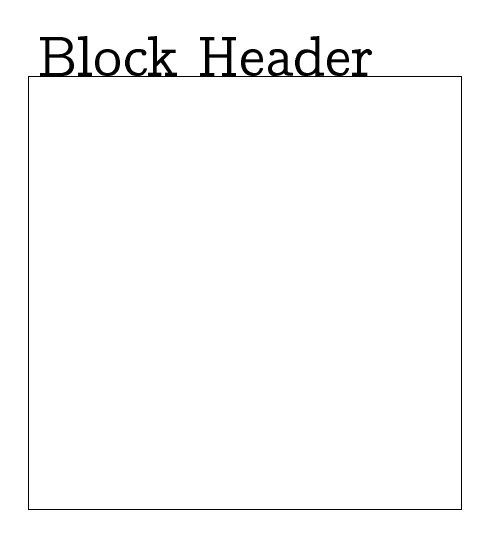
\begin{tikzpicture}
	\draw (0,0) rectangle (5.5,5.5);
	\draw (2.25,5.75) node {\huge{Block Header}};
\end{tikzpicture}
\printbibliography
\end{document}

